\documentclass[dvipsnames, svgnames, x11names, 11pt, twocolumn]{article}

\setlength{\columnsep}{20pt}

\usepackage[paper=a3paper, top=3cm, bottom=4cm, right=3.3cm, left=3.3cm]{geometry}

\usepackage{xcolor}
% URLs and hyperlinks ------------------------------
\usepackage{hyperref}
\hypersetup{
    colorlinks=true,
    linkcolor=DarkBlue,
    filecolor=magenta,
    urlcolor=blue,
}
\usepackage{xurl}
%---------------------------------------------------

\usepackage{caption}
\captionsetup{size=scriptsize}

\usepackage{graphicx}
\usepackage{float}
\usepackage{xepersian}
\settextfont{Yas}

\title{پاسخ تمرین اول درس کسب و کار}
\author{مهدی حق‌وردی}
\date{}

\begin{document}
\maketitle
\tableofcontents

\section{دلایل شکست هر استارت‌آپ را تحقیق و تحلیل کنید}
\subsection{آی‌هوم}
ایده‌ی کسب و کار آی‌هوم\RTLfootnote{که به دلیل علاقه‌ی موسس آن به محصولات اپل اینگونه نام‌گذاری شده است}
حدود سال‌های ۸۴ تا ۸۶ به ذهن آقا نیما\LTRfootnote{\url{https://virgool.io/product-management/@nima1980}} 
رسید و از سال ۸۷ شروع به فعالیت کرد.

نیما پا به بازاری گذاشته بود که طبق گفته‌های خودش
\begin{figure}[H]
\begin{center}

\includegraphics[width=0.45\textwidth, height=0.08\textheight]{images/market-size}
\caption{اندازه‌گیری‌های اولیه اندازه‌ی بازار املاک}
\end{center}
\end{figure}

\begin{figure}[H]
\begin{center}

\includegraphics[width=0.45\textwidth, height=0.08\textheight]{images/ms-2}
\caption{رشد خیلی خوب در شبکه‌ی اجتماعی فیس‌بوک}
\end{center}
\end{figure}

\begin{figure}[H]
\begin{center}

\includegraphics[width=0.45\textwidth, height=0.04\textheight]{images/ms-3}
\caption{تعداد ثبت‌نام‌ها و ورودی‌های سایت آی‌هوم}
\end{center}
\end{figure}

تا اینجا می‌توانیم نتیجه بگیریم که اتفاقا آی‌هوم روی بازار خیلی خوبی دست گذاشته بود و ساده‌تر:‌ مشتری داشت! پس نمی‌توان گفت که از دلایل شکست آی‌هوم کمبود بازار بود. اما آقا نیما یه کسب و کار دیگه‌ای به اسم پونیشا
\LTRfootnote{\url{https://ponisha.ir/}}
رو در حین داشتن آی‌هوم راه انداخت.

\begin{figure}[H]
\begin{center}
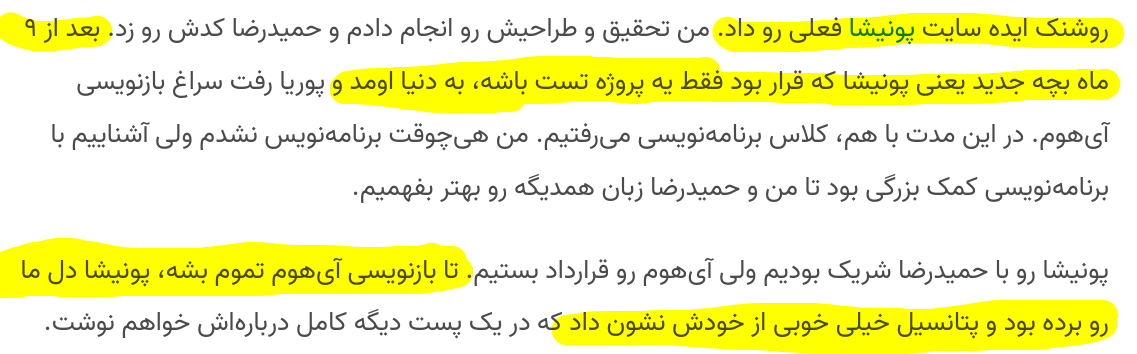
\includegraphics[width=0.45\textwidth, height=0.09\textheight]{images/ponisha-1}
\caption{راه‌اندازی پونیشا}
\end{center}
\end{figure}

و این یعنی کار فراوان و مدیریت دو تا بیزنس خیلی متفاوت
\begin{figure}[H]
\begin{center}
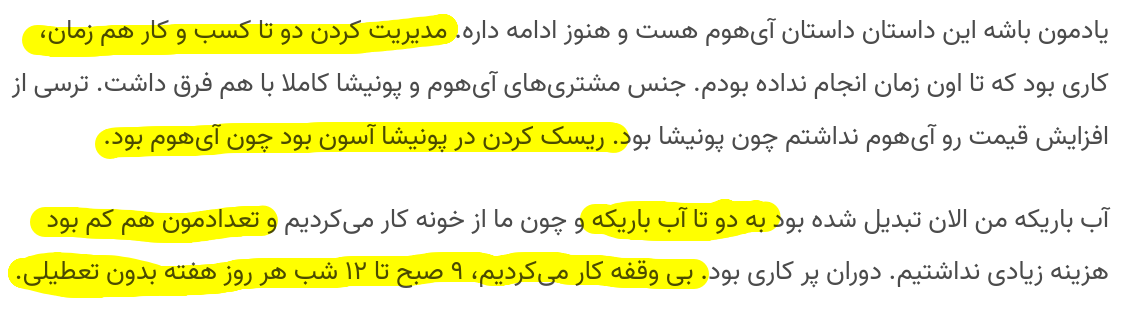
\includegraphics[width=0.45\textwidth, height=0.09\textheight]{images/ponisha-2}
\caption{مدیریت دو کسب و کار متفاوت و همزمان}
\end{center}
\end{figure}

و این شد که آقا نیما به فکر فروش آی‌هوم افتاد و با اینکه هنوز اون بیزنس مدل خیلی خوب رو شکل نداده بود

\begin{figure}[H]
\begin{center}
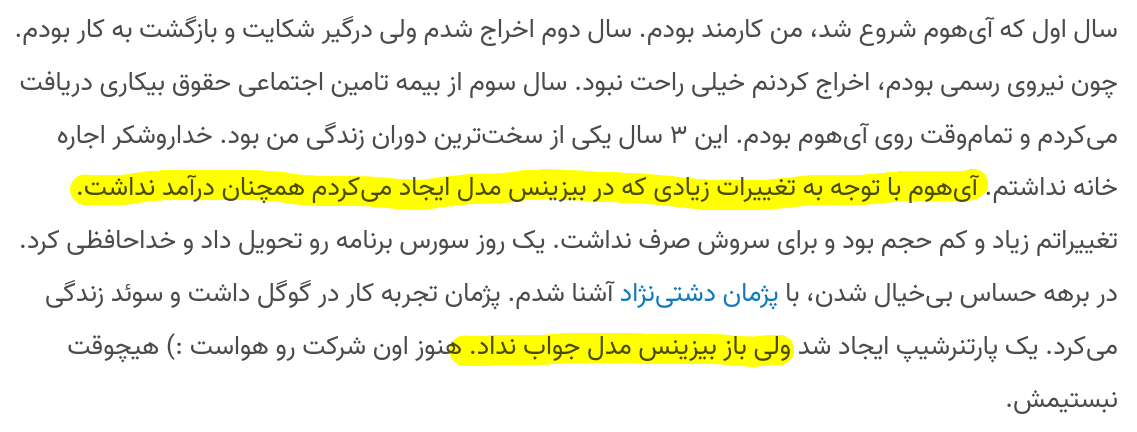
\includegraphics[width=0.45\textwidth, height=0.09\textheight]{images/business-model}
\caption{مدل‌های ناموفق کسب و کار آی‌هوم}
\end{center}
\end{figure}

پیشنهاد‌های خوبی هم گرفت

\begin{figure}[H]
\begin{center}

\includegraphics[width=0.45\textwidth, height=0.2\textheight]{images/buy-ihome}
\caption{پیشنهاد‌های خرید آی‌هوم}
\end{center}
\end{figure}
و در نهایت آقا نیما از شر آی‌هوم خلاص شد
\begin{figure}[H]
\begin{center}
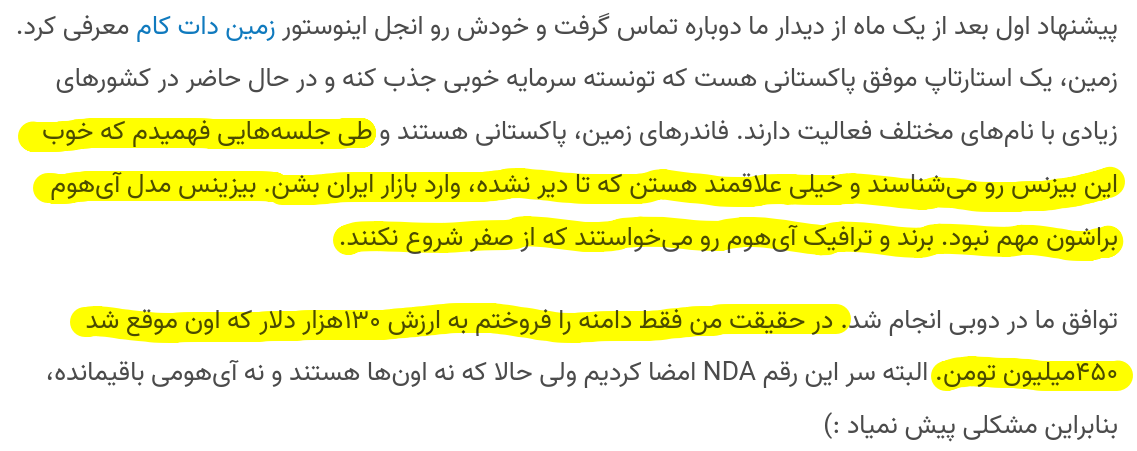
\includegraphics[width=0.45\textwidth, height=0.13\textheight]{images/sell-ihome}
\caption{فروش آی‌هوم}
\end{center}
\end{figure}

پس از فروش آی‌هوم، پاکستانی‌ها خوب تونسته بودن کسب و کار رو رشد بدن \textbf{اما سایه‌ی تحریم‌ها بالاخره اثر خودش رو گذاشت و کمر پاکستانی‌ها رو شکست}

\begin{figure}[H]
\begin{center}
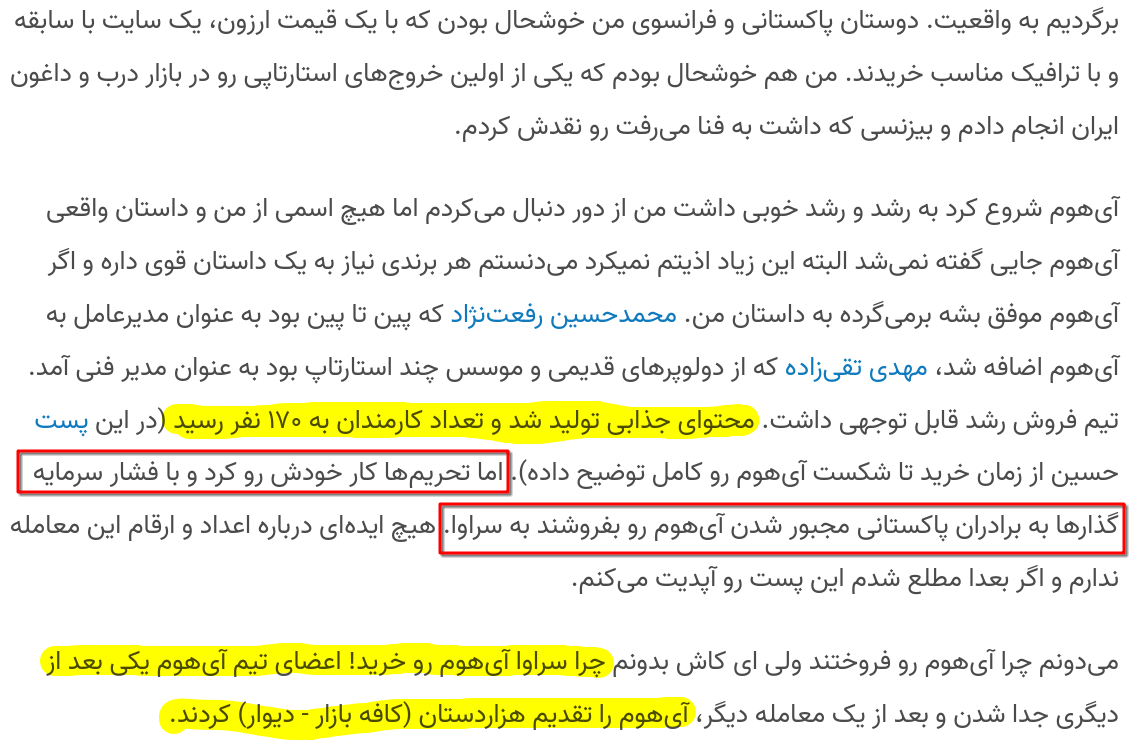
\includegraphics[width=0.45\textwidth, height=0.2\textheight]{images/sanctions}
\caption{فروش آی‌هوم}
\end{center}
\end{figure}

بعد از این خرید و فروش‌های آی‌هوم، در نهایت این کسب و کار درش بسته شد و میشه گفت دیوار تونست کمی از بازار اون رو بیاره توی پلتفرم خودش.

در نهایت میشه گفت: نداشت یه تیم تحقیق و توسعه‌ی قوی، تحریم‌ها و مدیریت نادرست و تضاد منافع باعث شد که آی‌هوم سرش رو بذاره زیر گِل.

\subsubsection{منابع}
\begin{itemize}
\item 
\url{https://nakamology.ir/projects/ihome/}

\item 
\href{https://virgool.io/product-management/%D8%AF%D8%A7%D8%B3%D8%AA%D8%A7%D9%86-%D8%A2%DB%8C-%D9%87%D9%88%D9%85-%D8%B4%D8%B1%D9%88%D8%B9-%D9%85%D9%88%D9%81%D9%82%DB%8C%D8%AA-%D9%88-%D8%B4%DA%A9%D8%B3%D8%AA-aoxc2pqljwbu}{\lr{\texttt{https://virgool.io/product-management/}}داستان-آی-هوم}

\item 
\url{https://www.zoomit.ir/tech-iran/339825-divar-acquired-ihome/}
\end{itemize}

\subsection{\lr{argyled}}
این کسب و کار یک پلتفرم مدیریت شبکه‌های اجتماعی برای کسب و کار‌های دیگر بود. این یعنی مدل کسب و کاری این پلتفرم به صورت
\lr{B2B}
بود.

این کسب و کار طراحی، تجربه‌ی کاربری و فیچر‌های خیلی خوبی ارائه می‌داد اما متاسفانه بخاطر اندازه‌ی کوچک‌تر نسبت به کسب و کار‌های خیلی بزرگ‌تر از خودش در رقابت دوام نیاورد

\begin{figure}[H]
\begin{center}
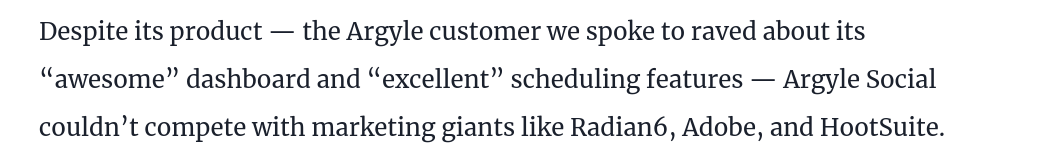
\includegraphics[width=0.5\textwidth, height=0.05\textheight]{images/argyle-ui}
\caption{طراحی عالی و فیچر‌های جذاب، اما رقیب‌های بزرگ}
\end{center}
\end{figure}

به علاوه \textbf{زیاد و پیچیده بودن روند توسعه} هم (بخاطر اینکه شرکت کوچکی بودند و توسعه‌دهنده‌های کمی داشتند) باعث عقب ماندن و رشد کند این کسب و کار شد

\begin{figure}[H]
\begin{center}
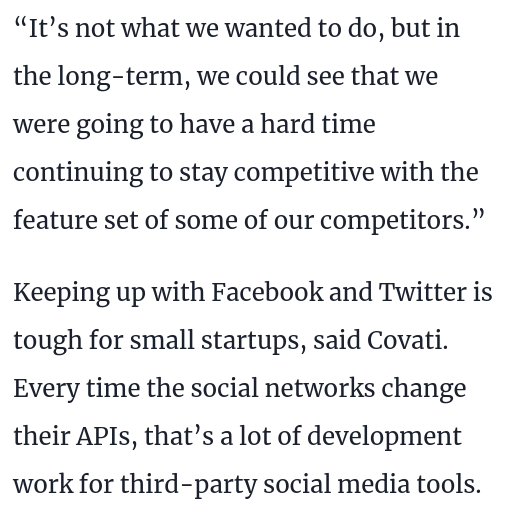
\includegraphics[width=0.3\textwidth, height=0.25\textheight]{images/argyle-twitter}
\caption{سختی این صنعت و هزینه‌ی توسعه‌ی زیاد}
\end{center}
\end{figure}

در نهایت می‌شود گفت: رقیب‌های بزرگ و کوچک بودن تیم و سخت بودن ذاتی این صنعت باعث شد که 
\lr{argyle}
هم به زیر گِل هُل داده شود.

\subsubsection{منابع}
\begin{itemize}
\item 
\url{https://startupgraveyard.io/company/argylesocial/}

\item 
\url{https://startupgraveyard.io/company/argylesocial/}
\end{itemize}


\section{از نگاه شما، مواردی که در سایت ذکر نشده‌اند، چه دلایل دیگری باعث شکست این کسب و کار‌ها شده است؟}
\subsection{آی‌هوم}
تجربه‌ی اولی بودن و شروع در زمانی که کسب و کار آنلاین خیلی مطرح نبوده هم می‌تواند از دلایل شکست این کسب و کار باشد؛ به این دلیل که آی‌هوم کاملا آنلاین بود و کسب و کار نویی در زمان خودش محسوب می‌شد.

\subsection{\lr{argyle}}
به نظر من اگر مثل تلگرام که در بازاری که هم واتساپ وجود داشت و هم فیس‌بوک مسنجر، اگر می‌توانستند سرمایه‌گذار پیدا کنند و بار کاری و فشار رقیبان را تحمل کنند، ممکن بود موفق بشوند. بنظرم کنار کشیدن و نداشتن سرمایه‌گذار‌های جدید از دلایل دیگر این کسب و کار‌ها بود.

\section{با توجه به دلایل شناسایی شده، اگه شما جای مدیر آن کسب و کار بودید، چه اقداماتی برای پیشگیری انجام می‌دادید؟ حداقل دو مورد ذکر کنید.}
\subsection{آی‌هوم}
\begin{enumerate}
\item 
پیدا کردن فاندر‌های دیگر کسب و کار‌ها و نوشتن یک مدل کسب و کاری بهتر از ابتدا برای آی‌هوم

\item 
استفاده و ریسک کردن با پشتیبانی از پونیشا برای چند وجهی کردن آی‌هوم

\end{enumerate}

\subsection{\lr{argyle}}
\begin{enumerate}
\item 
صحبت با رقیبان برای ادغام شرکت در شرکت آنها (مثل ادغام شدن مارول و پیکسار در دیزنی)

\item 
بستن قرارداد با شبکه‌های اجتماعی برای گرفتن 
\lr{endpoint}های 
اختصاصی 
\end{enumerate}

\section{حداقل یک رقیب مستقیم یا غیر مستقیم برای این کسب و کارها مثال بزنید که به موفقیت رسیده‌اند (علت موفقیت را هم تحلیل کنید).}
\subsection{آی‌هوم}
دیوار

کسب و کار دیوار به دلیل داشتن پشتوانه‌ی اساسی و بزرگ، همچنین داشتن مدل کسب و کاری خوب از ابتدا به علاوه چند وجهی بودن کسب و کار توانست که موفق بشود، و هم‌اکنون هم بسیاری از معاملات مسکن در دیوار انجام می‌شوند.

\subsection{\lr{argyle}}
\lr{sprinklr}

بنظرم علت موفقیت این کسب اینست که توانسته با شرکت‌های واقعا بزرگ 
\begin{figure}[H]
\begin{center}

\includegraphics[width=0.5\textwidth, height=0.05\textheight]{images/argyle-big}
\caption{همکاری با شرکت‌های بزرگ}
\end{center}
\end{figure}
همکاری داشته باشد.

این باعث می‌شود که هم پول ورودی بیشتری داشته باشد تا بتواند توسعه‌دهنده‌های بیشتری را استخدام کند، و هم باعث تبلیغات بزرگی برای این شرکت می‌شود.

به علاوه این شرکت توانسته سرمایه‌ی خیلی خوبی را جمع می‌کند
\begin{figure}[H]
\begin{center}

\includegraphics[width=0.5\textwidth, height=0.05\textheight]{images/sp-fund}
\caption{جمع‌آوری سرمایه‌ی عظیم}
\end{center}
\end{figure}

\begin{figure}[H]
\begin{center}

\includegraphics[width=0.5\textwidth, height=0.05\textheight]{images/sp-fund-2}
\caption{جمع‌آوری سرمایه‌ی عظیم}
\end{center}
\end{figure}

همچنین بروز بودن این شرکت با تغییرات دنیای تکنولوژی 
\begin{figure}[H]
\begin{center}

\includegraphics[width=0.5\textwidth, height=0.05\textheight]{images/sp-ai}
\caption{استفاده از هوش مصنوعی در محصولات}
\end{center}
\end{figure}

همه و همه باعث شده این کسب و کار نتیجه‌ی بهتری از 
\lr{argyle social}
بگیرد.

\end{document}